\documentclass[11pt,letterpaper]{article}
\usepackage{emnlp2016}
\usepackage[utf8]{inputenc}
\usepackage{times}
\usepackage{url}
\usepackage{latexsym}
\usepackage{amsmath}
\usepackage{amsfonts}
\usepackage{graphicx}
%\emnlpfinalcopy

%  Enter the EMNLP Paper ID here:
\def\emnlppaperid{***}

%\setlength\titlebox{5cm}

% How about this:
\title{Levels of representation in a Stacked Gated Recurrent Neural
  Network model of visually-grounded language learning}
\author{Lieke Gelderloos \\
  Tilburg University \\
  {\tt l.j.gelderloos@uvt.nl} \And
  Grzegorz Chrupa?a \\
  Tilburg University \\
  {\tt g.chrupala@uvt.nl} }

\date{}

\begin{document}
\maketitle
\begin{abstract}
Language learning children discover both the structure of language and the ways in which it relates to the world from continuous perceptual data in different modalities. We present {Phoneme GRU}, an architecture composed of stacked Gated Recurrent Units that learns to predict visual features given an image caption in the form of a sequence of phonemes. Although the language input consists of low-level symbolic input rather than a continuous speech signal, the learning task resembles that human language learners in the sense that the learner learns both structure and meaning from noisy and ambiguous data. We show that {\sc Phoneme GRU} indeed learns to predict features of the visual context given phonetically transcribed image captions, and show that it represented linguistic structure in a hierarchical manner: lower layers in the stack are comparatively more sensitive to form, whereas higher layers are more sensitive to meaning.

\end{abstract}

\section{Introduction}
\label{sec:intro}
% I think this first paragraph needs the word 'grounded/ing' somewhere
Children acquire their native language with little and weak
supervision, exploiting noisy correlations between speech, visual, and
other sensory signals, as well as via feedback from interaction with
their peers and parents. Understanding this process is an important
scientific challenge in its own right, but it also has potential to
generate insights useful in engineering efforts to design
conversational agents or robots. Computationally modeling the ability
to learn linguistic form--meaning pairings has been the focus of much
research, under scenarios simplified in a variety of ways, for
example:

\begin{itemize}
\item distributional learning from pure word-word co-occurrences with
  no perceptual grounding \cite{landauer1998introduction,kiros2015skip};
\item cross-situational learning with word sequences and sets of
  symbols representing sensory input
  \cite{siskind.96,fazly.etal.10csj};
\item cross-situational learning using sensory audio and visual
  input, but with extremely limited sets of words and objects
  \cite{Roy2002113,iwahashi2003language}.
\end{itemize}

Some recent models have used more naturalistic, larger-scale inputs,
for example in cross-modal distributional semantics
\cite{lazaridou2015combining} or in implementations of the acquisition
process trained on images paired with their descriptions
\cite{chrupala2015learning}. While in these works the representation
of the {\it visual scene} consists of pixel-level perceptual data, the
{\it linguistic} input consists of sentences segmented into discrete
word symbols. In this paper we take a step towards addressing this
major limitation, by using the phonetic transcription of input
utterances. While this type of input is symbolic rather than
perceptual, it goes a long way toward making the setting more
naturalistic, and the acquisition problem more challenging: the
learner may need to discover structure corresponding to morphemes, words
and phrases in an unsegmented string of phonemes, and the length of
the dependencies that need to be detected grows substantially when
compared to word-level models.

\paragraph{Our contributions}

We design and implement a simple architecture based on stacked
recurrent neural networks with Gated Recurrent Units
\cite{chung2014empirical}: our model processes the utterance phoneme
by phoneme while building a distributed low dimensional representation
through a series of recurrent layers. Once it reaches the end of the
utterance it attempts to predict the features of the corresponding
visual scene. We train this model on a phonetically transcribed
version of MS-COCO \cite{lin2014microsoft} and show that it is able to
successfully learn to understand aspects of sentence meaning from the
visual signal, and exploits temporal structure in the input. In a
number of experiments we show that different levels in the stack of
recurrent layers represent different aspects of linguistic
structure. Low levels focus on local, short time-scale portions of the
input sequence, and are comparatively more sensitive to form. The top
level encodes global aspects of the input sequence and is sensitive to
visually salient elements of its meaning.

\section{Related work}
% kleine zin om te zeggen waar je het aan gaat relateren?

In language acquisition research, grounded learning of (sometimes combined) word learning and word segmentation is often studied in the cross-situational learning paradigm. %you should probably extend this somewhat & mention some experimental work. also that sentence is really ugly.
Two computational models that take the continuous nature of the speech signal into account, as well as incorporating visual information, are the Cross-channel Early Lexical Learning (CELL) model of \newcite{Roy2002113} and the more recent work of \newcite{rasanen2015joint}. The CELL model aims to discover words from continuous speech and learn their meaning, but is very limited with regards to visual input, which only consists of the shape of single objects in the visual context. \newcite{rasanen2015joint} propose a probabilistic joint model of word segmentation and meaning acquisition from raw speech and visual context. The visual context in this model consists of a collection of possible referents present in the environment, making it richer than the visual input in CELL, but also abstracting away further from the raw visual data. 

There is an extensive line of research in automatic image captioning (see \newcite{bernardi2016automatic} for a recent overview). Typically, image captioning models learn to recognize high-level image features and associate them with words. Inspired by both image captioning research and cross-situational human language acquisition, two recent Automatic Speech Recognition models learn to recognize word forms from visual data. In \newcite{synnaeve2014learning}, language input consists of single spoken words and visual data consists of image fragments, which the model learns to associate. \newcite{harwath2015deep} employ two convolutional neural networks, a visual object recognition model and a word recognition model, and an embedding alignment model that learns to map recognized words and objects into the same high-dimensional space. Although the object recognition works on the raw visual input, the speech signal is segmented into words before presenting it to the word recognition model. Whereas in \newcite{harwath2015deep} the visual input only plays a role at the utterance level, and not at the sub-word level, \newcite{synnaeve2014learning} only consider the (sub)-word level and do not look at the larger utterance context. 

Character-level language models are described and interpreted in \newcite{hermans2013training} and \newcite{karpathy2015visualizing}. Both studies show that character-level deep recurrent neural networks are sensitive to long-range dependencies: for example by keeping track of opening and closing parentheses over long stretches of text. \newcite{hermans2013training} describe the somewhat hierarchical organization that seems to emerge during training, with higher layers processing information over linger timescales. In our work we show related effects in the context of a model of visually-grounded language learning from unsegmented phonetic strings.

In the current study we use phonetic transcription of full sentences as a first step towards large-scale multimodal language learning from speech co-occurring with visual scenes. In contrast to \newcite{Roy2002113} and \newcite{rasanen2015joint}, the visual input to our model consists of high-level visual features, which means it contains ambiguity and noise. In contrast to \newcite{synnaeve2014learning} and  \newcite{harwath2015deep}, we consider full utterances rather than separate words. To our knowledge, there is no work yet on multimodal phoneme or character-level language modeling with visual input. Our study is complementary to work on character-level language modeling: while language models focus on {\it within}-text co-occurrence statistics as clues to language structure, in our setting the weight is on the correlations  {\it between} language and the visual scenes. Although the language input in this study is low-level-symbolic rather than perceptual, the learning problem we aim to solve is similar to that of a human language learner: the learner has to discover language structure as well as meaning, based on ambiguous and noisy data from another modality.  

\newcite{chrupala2015learning} simulate visually grounded human language learning with specific sensitivity to the noise and ambiguity in the visual domain. They model language learning as a task of predicting visual context given a sequence of words. While the visual input consists of a continuous representation, the language input consists of a sequence of words. The aim of this study is to take their approach one step further towards multimodal language learning from raw perceptual input. 

\newcite{Kdr2016RepresentationOL} develop techniques for understanding, interpretation and visualization of the representations of linguistics form and meaning in recurrent neural networks, and apply these to word-level models. In our work we share the goal of revealing the nature of emerging representations, but we do not assume words and word embeddings as their basic unit. Also, we are especially concerned with the emergence of a hierarchy of levels of representations in stacked recurrent networks.


\section{Models}
\label{sec:models}

\subsection{Phoneme Stacked GRU}
The architecture of our main model of interest, {\sc Stacked GRU} is
schematically depicted in Figure \ref{fig:architecture} and consists of a phoneme
encoding  layer, followed by a stack of $K$ Gated Recurrent Neural
nets, followed by densely connected layer which maps the last hidden
state of the top recurrent layer to a vector of visual features.

\begin{figure}
  \centering
  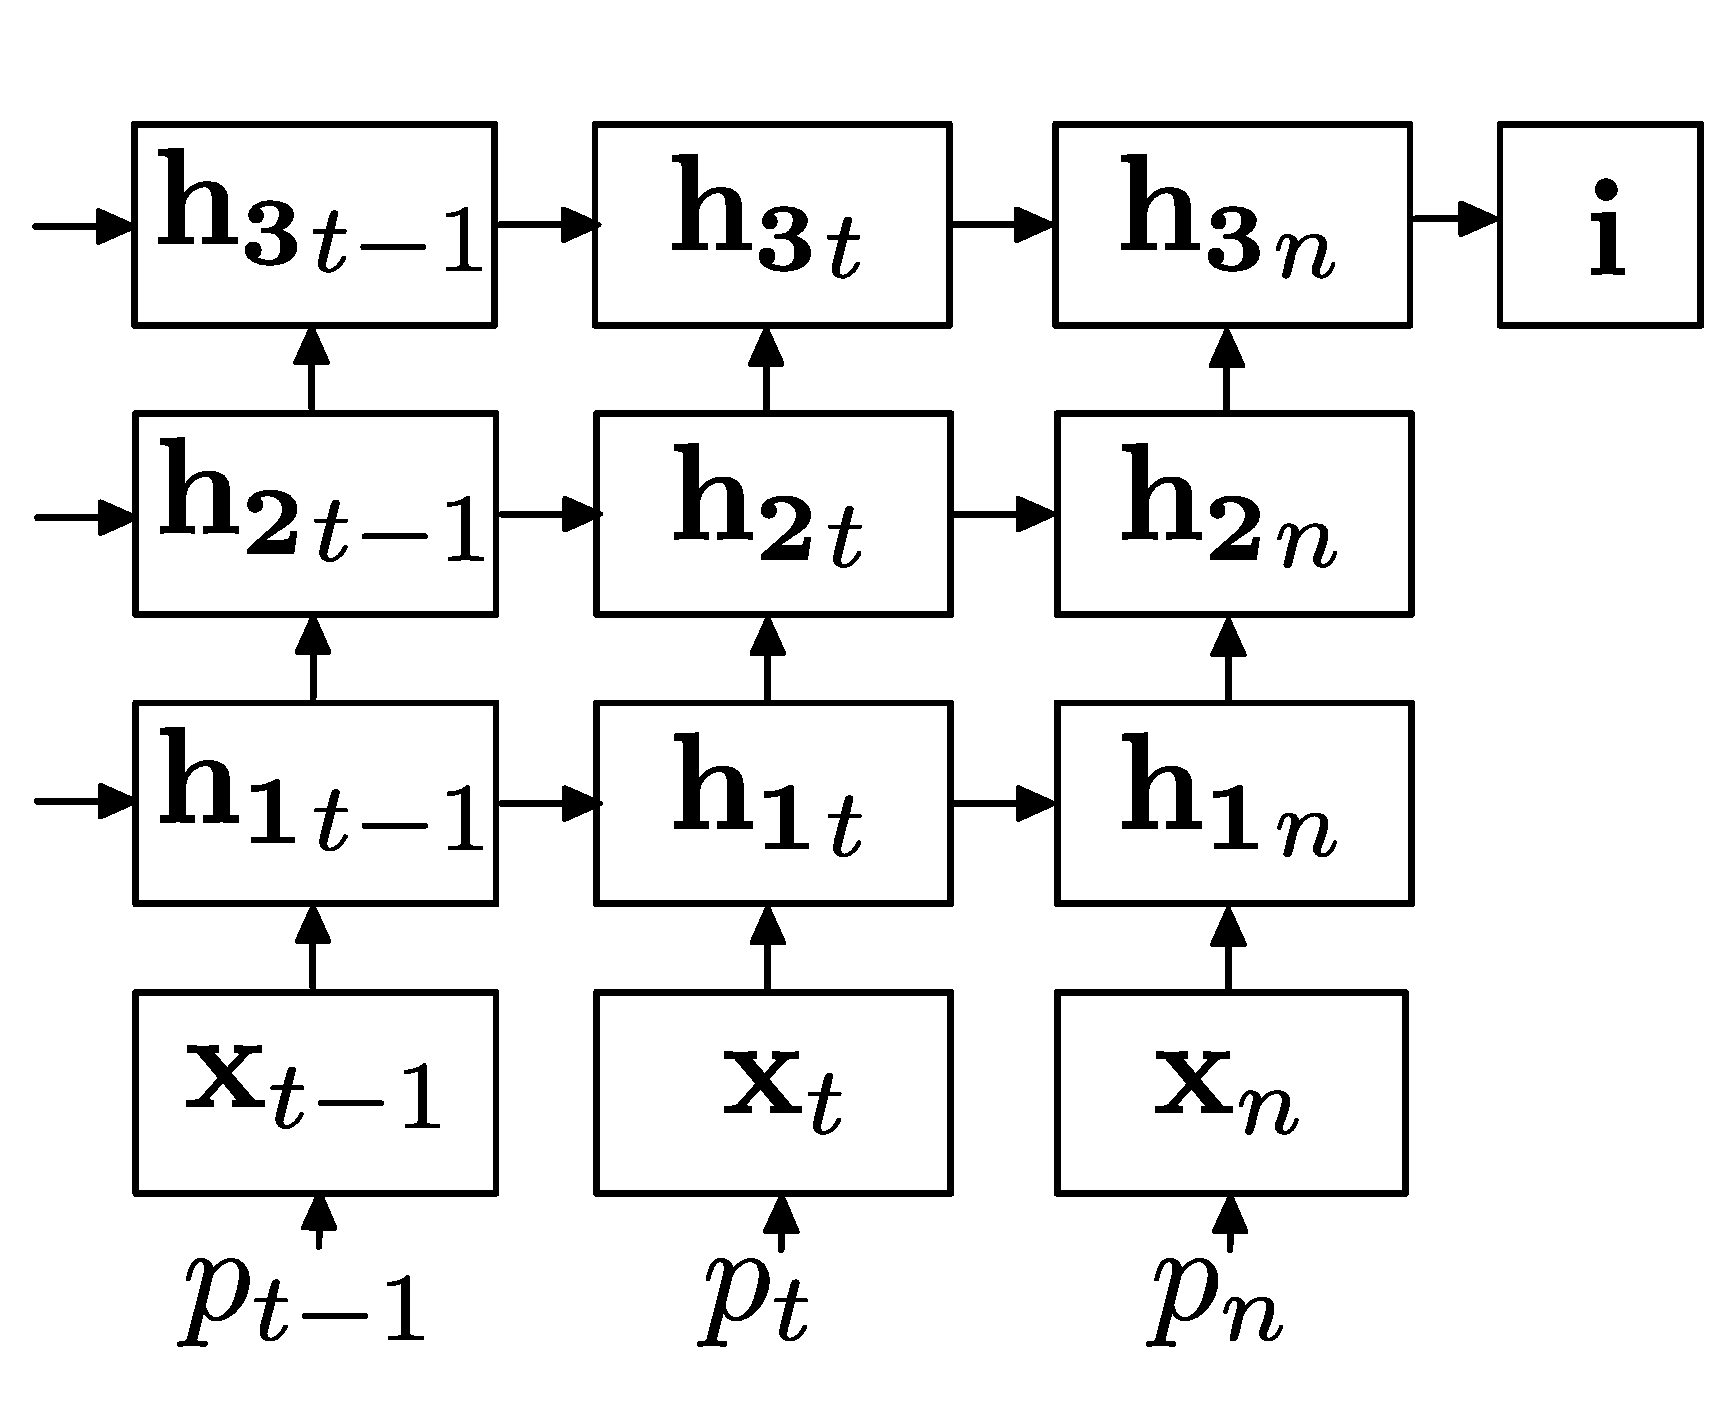
\includegraphics[scale=0.2]{architecture.pdf}
  \caption{A three-timestep slice of the stacked recurrent architecture with three hidden layers.}
  \label{fig:architecture}
\end{figure}

Gated Recurrent Units (GRU) were introduced in
\newcite{cho2014properties} and \newcite{chung2014empirical} as an
attempt to alleviate the problem of vanishing gradient in standard
simple recurrent nets as known since the work of
\newcite{elman1990finding}. GRUs have a linear shortcut through
timesteps which bypasses the nonlinearity and thus promotes gradient
flow.
Specifically, a GRU computes the hidden state at current time step, $\mathbf{h}_{t}$, as the
linear combination of previous activation $\mathbf{h_{t-1}}$, and a new
{\it candidate} activation $\mathbf{\tilde{h}}_t$:
%

\begin{equation}
  \mathrm{gru}(\mathbf{x}_t, \mathbf{h}_{t-1}) = (1 - \mathbf{z}_t)\odot \mathbf{h}_{t-1} + \mathbf{z}_t \odot \mathbf{\tilde{h}}_t
\vspace{-.1cm}
\end{equation}
%
where $\odot$ is elementwise multiplication, and the update gate
activation $\mathbf{z_{t}}$ determines the amount of new information
mixed in the current state:
%

\begin{equation}
\label{eq:gru-update}
   \mathbf{z}_t = \sigma_s(\mathbf{W}_z \mathbf{x}_t + \mathbf{U}_z \mathbf{h}_{t-1})
\end{equation}
%
The candidate activation is computed as:
%
\begin{equation}
\label{eq:gru-cand}
   \mathbf{\tilde{h}}_t = \sigma(\mathbf{W} \mathbf{x}_t + \mathbf{U}(\mathbf{r}_t \odot \mathbf{h}_{t-1}))
\end{equation}
%
The reset gate $\mathbf{r_{t}}$ determines how much of the current
input $\mathbf{x_{t}}$ is mixed in the previous state
$\mathbf{h}_{t-1}$ to form the candidate activation:
%
\begin{equation}
\label{eq:gru-reset}
   \mathbf{r}_t = \sigma_s(\mathbf{W}_r \mathbf{x}_t + \mathbf{U}_r \mathbf{h}_{t-1})
\end{equation}

By applying the $\mathrm{gru}$ function repeatedly a GRU layer maps a
sequence of inputs to a sequence of states:
\begin{equation}
  \mathrm{GRU}(\mathbf{X}, \mathbf{h}_0) = \mathrm{gru}(\mathbf{x}_n, \dots, \mathrm{gru}(\mathbf{x}_2, \mathrm{gru}(\mathbf{x}_1, \mathbf{h}_0)))
\end{equation}
where $\mathbf{X}$ stands for the matrix composed of input column vectors
$\mathbf{x}_1, \ldots, \mathbf{x}_n$. Two or more GRU layers can be composed into a stack: 
\begin{equation}
\mathrm{GRU}_2(\mathrm{GRU}_1(\mathbf{X}, {\mathbf{h}_{0}}_{1}), {\mathbf{h}_{0}}_{2}).
\end{equation}
In our version of the Stacked GRU architecture we use {\it residualized} layers:
\begin{equation}
\mathrm{GRU_{res}}(\mathbf{X}, \mathbf{h}_0) = \mathrm{GRU}(\mathbf{X}, \mathbf{h}_0) + \mathbf{X}
\end{equation}
Residual convolutional networks were introduced by
\newcite{he2015deep}, while \newcite{oord2016pixel} showed their
applicability to recurrent architectures. We adopt residualized layers
here are we observed they speed up learning in stacks of several
GRU layers.

Our gated recurrent units use steep sigmoids for gate activations: \[
\sigma_s(z) = \frac{1}{1 + \exp(-3.75z)} 
\]
and rectified linear units clipped between 0 and 5 for the unit
activations:
\[
\sigma(z) = \mathrm{clip(0.5(z+\mathrm{abs}(z)), 0, 5)}
\]

There are two more components of our {\sc Stacked GRU} model: the
phoneme encoding layer, and mapping from the final state of the top GRU
layer to the image feature vector.
The phoneme encoding layer is a simply a lookup table $\mathbf{E}$ whose
columns correspond to one-hot-encoded phoneme vectors. The input
phoneme $p_t$ of utterance $p$ at each step $t$ indexes into the
encoding matrix and produces the input column vector:
\begin{equation}
  \mathbf{x}_t = \mathbf{E}[:,p_t].
\end{equation}
Finally, we map the final state of the top GRU layer ${\mathbf{h}_K}_n$
to the vector of image features using a fully connected layer:

\begin{equation}
  \hat{\mathbf{i}} = \mathbf{I} {\mathbf{h}_K}_n
\end{equation}

Our main interest lies in  recurrent phoneme-level modeling. However in order to
put the performance of the phoneme-level {\sc Stacked GRU} into
perspective we compare it to the following two other models.


\subsection{Word GRU}
The architecture of this model is the same as {\sc Stacked GRU} with
the difference that we use words instead of phonemes as input symbols,
use learnable word embeddings instead of fixed on-hot phoneme
encodings, and reduce the number of layers in the GRU stack. See
\ref{sec:experiments} for details.
\subsection{Word Vector Sum}
The second model we use for comparison is word-based non-sequential
model, consisting of a word embedding matrix, a vector sum operator,
and a mapping to the image vector feature vector:
\begin{equation}
  \label{eq:sum}
  \hat{\mathbf{i}} = \mathbf{I} \sum_{t=1}^n \mathbf{E}[:,w_t]
\end{equation}
where $w_t$ is the word at position $t$ in the input utterance.
This model simply learns word embeddings which are then summed into a
single vector and projected to the target image vector. Thus this model does
not have access to word sequence information, and is a distributed
analog of a bag-of-words model.

\section{Experiments}
\label{sec:experiments}

For all experiments, the models were trained on the training set of MS-COCO. MS-COCO contains over 163,000 images accompanied by at least five captions by human annotators. With an average of 7.7 labeled object instances per image, images typically contain more objects than the captions mention, making reference to the scene ambiguous. Textual input for the {\sc Phon GRU} models was transcribed automatically using the grapheme-to-phoneme functionality with the default English voice of the eSpeak speech synthesis toolkit.\footnote{Available at \url{http://espeak.sourceforge.net}} Stress and pause markers were removed, as well as word boundaries (after storing their position for use in experiments), leaving only phoneme symbols. See Figure~\ref{fig:ipa} for an example transcription.


Visual input for all models was obtained by forwarding images through the 16-layer convolutional neural network described in \newcite{simonyan2014very} pre-trained on Imagenet \cite{ILSVRCarxiv14}, and recording the activation vectors of the pre-softmax layer. The z-score transformation was applied to these features to ease optimization. 

Most of the details of the three model types and training
hyperparameters were adopted from related work, and adapted via
a limited amount of exploratory experimentation. Exhaustive exploration of the search space was not feasible due to the large number of adjustable settings in these models and their long running time. Given the importance of depth for our purposes, we did systematically explore the number of layers in the {\sc Phon GRU} and {\sc Word GRU} models. A single layer is optimal for {\sc Word GRU}. For {\sc Phon GRU}, see Section~\ref{subsec:visual} below. Other important settings were as follows:
\begin{itemize}
\setlength\itemsep{-0.5em}
\item All models: Implemented in Theano \cite{Bastien-Theano-2012}, optimized with 
  Adam \cite{DBLP:journals/corr/KingmaB14}, initial learning rate of 0.0002, minibatch size
  of 64, gradient norm clipped to 5.0.
\item {\sc Word Sum}: 1024-dimensional word embeddings, words with frequencies below 10 replaced by {\tt UNK} token.
\item {\sc Word GRU}: 1024-dimensional word embeddings, a single 1024 dimensional hidden layer, words with frequencies below 10 replaced by {\tt UNK} token.
\item {\sc Phon GRU}: 1024-dimensional hidden layers.
\end{itemize}

\subsection{Prediction of visual features}
\label{subsec:visual}
The models are trained and evaluated on the prediction of visual
feature vectors from captions. While our goal is not to develop an
image retrieval method, we use this this task as it reflects the ability to extract visually salient semantic information from language.
For the experiments on the prediction of visual features all models
were trained on the training set of MS COCO. As validation and test data we
used a random sample of 5000 images each from the MS COCO validation set. 

Figure~\ref{fig:loss} shows the value of the validation average cosine distance
between the predicted visual vector and the target vector for three
random initializations of each of the model types. 

The Phonetic GRU model is more sensitive to the initialization: one
can clearly distinguish three separate trajectories. The word-level models
are much less affected by random initialization. In terms of the
overall performance, the {\sc Phon GRU} model falls between the
{\sc Word Sum} model and the {\sc Word GRU} model.

\begin{figure}
    \centering
  \begin{minipage}{0.45\textwidth}
    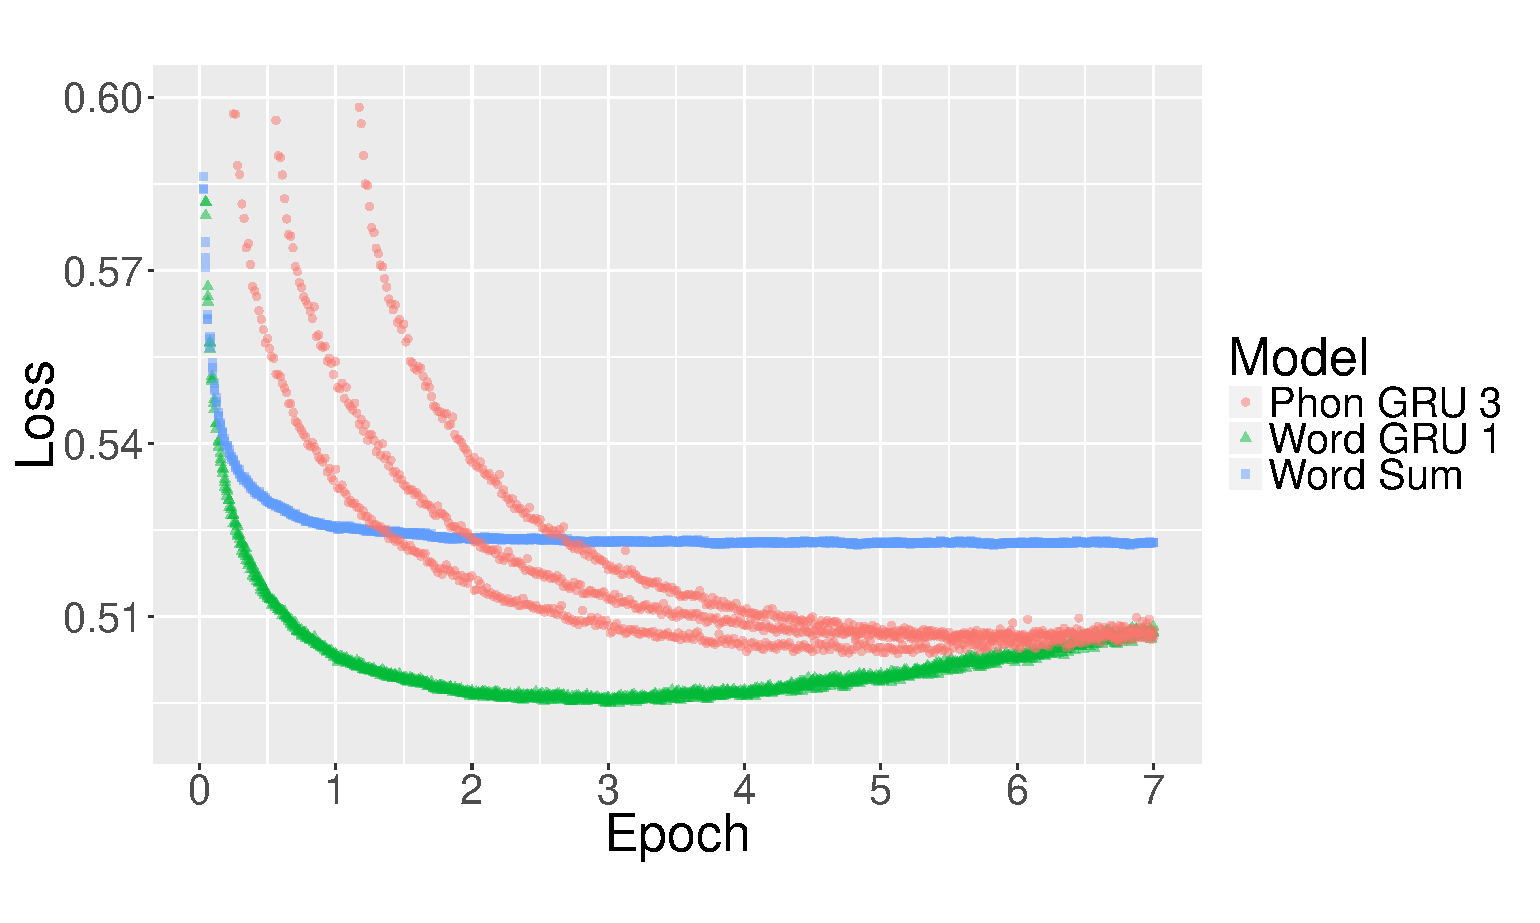
\includegraphics[scale=0.32]{loss-zoom.pdf}
    \caption{Value of the loss function on validation data during
      training. Three random initialization of each model are shown.}
    \label{fig:loss}
  \end{minipage}
\hspace{0.3cm}
  \begin{minipage}{0.45\textwidth}
    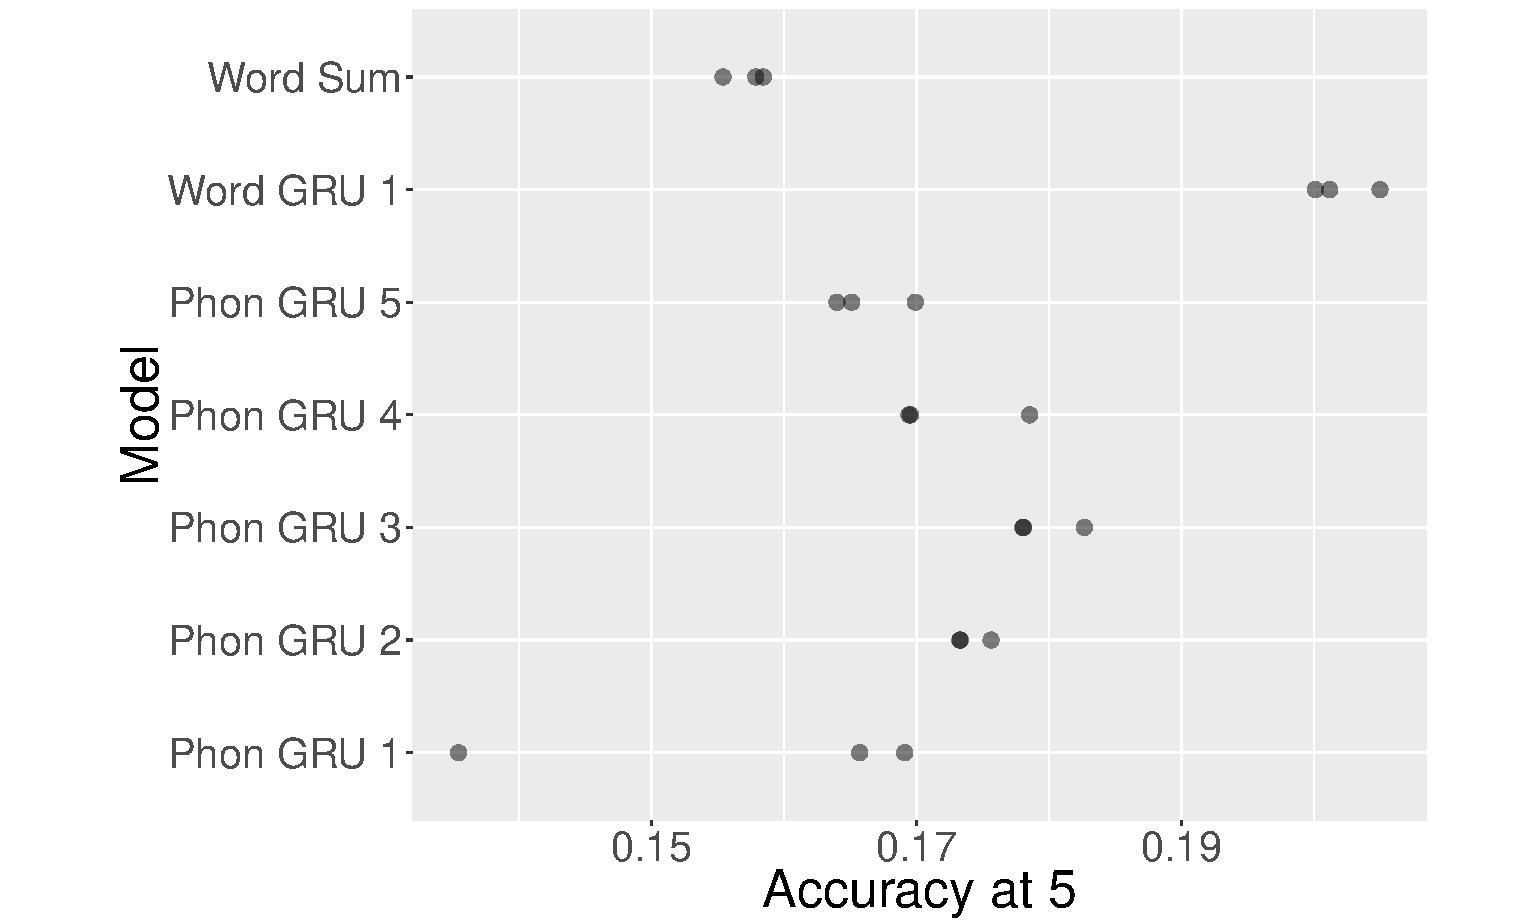
\includegraphics[scale=0.32]{accat5.pdf}
    \caption{Validation accuracy at 5 on the image retrieval task.}
    \label{fig:accat5}
  \end{minipage}
\end{figure}

We also evaluated the models on how well they perform when used to
search images: for each validation sentence the model was used to predict the
visual vector. The image vectors in the validation data were then
ranked by cosine similarity to the predicted vector, and the
proportion of times the correct image was among the top 5 was
reported. By {\it correct} image we mean the one which the sentence
was used to describe (even though often many other images are also
good matches to the sentence). 

In Figure~\ref{fig:accat5} we report the validation accuracies on this
task for the two word-level models, as well as for the Phon GRU
model with different number of hidden layers. We trained each model
version with three random initializations for each model setting, and
evaluate after each epoch. We report the score of the best epoch for
each initialization. 
The overall ranking of the models matches the direct
evaluation of the loss function above: the phoneme-level models are in
between the two word-level models. {\sc Phon GRU} with three
hidden layers is the best of the phoneme-level models.

In Table~\ref{tab:accat5test} we show the accuracies of the best
version of each of the models types on the test images; these are also
the model versions used in all subsequent experiments. The accuracy @
5 for the {\sc Word GRU} is comparable to what
\newcite{chrupala2015learning} report for their multitask {\sc
  Imaginet} model, whose visual pathway has the same
structure. \newcite{vendrov2015order} report substantially higher
scores for image search with a word level GRU model, with the
following main differences from our setting: better image features,
larger training set, and a loss function optimized for the ranking
task.\footnote{We have preliminary results indicating that most of the
  analyses in the rest of Section~\ref{sec:experiments} show the same general
  pattern for phoneme models trained following the setting of
  \newcite{vendrov2015order}.}.

% \begin{table}
%   \centering
%   \begin{tabular}{ll|r}
%  Model     & Layers & Acc. at 5 \\\hline
%  Word Sum  & 0      & 0.158 \\
%  Word GRU  & 1      & 0.205 \\\hline
%  Phon GRU  & 1      & 0.169  \\
%  Phon GRU  & 2      & 0.176  \\
%  Phon GRU  & 3      & \bf 0.183  \\  
%  Phon GRU  & 4      & 0.179 \\
%  Phon GRU  & 5      & 0.170 \\
%   \end{tabular}
% \caption{Accuracy at 5 on the image retrieval task.}
% \label{tab:accat5}
% \end{table}

\subsection{Word boundary prediction}
To explore the sensitivity of the {\sc Phon GRU} model to linguistic structure at the sub-word level, we investigated the encoding of information about word-boundaries in the hidden layers. Logistic regression models were trained on activation patterns of the hidden layers at all timesteps, with the objective of identifying phonemes that preceded a word boundary. For comparison, we also trained logistic regression models on \textit{n}-gram data to perform the same tasks, with positional phoneme \textit{n}-grams in the range $1$-\textit{n}. The location of the word boundaries was taken from the eSpeak transcriptions, which mostly matches the location of word boundaries according to conventional English spelling. However, eSpeak models some coarticulation effects which sometimes leads to word boundaries disappearing from the transcription. For example, {\it bank of a river} is transcribed as \textipa{[baNk @v@ \*rIv@]}.

All models were implemented using the {\tt LogisticRegression} implementation from Scikit-learn \cite{scikit-learn} with L2-regularization. The random samples of 5,000 images each that served as validation and test sets in the visual feature prediction task were used as training and test sets. The optimal value of regularization parameter \textit{C} was determined using {\tt GridSearchCV} with 5-fold cross validation on the training set, after which the model with the optimal settings was trained on the full training sample.

Table~\ref{tab:boundary} reports the scores on the test set. The proportion of phonemes preceding a word boundary is 0.29, meaning that predicting {\it no word boundary} by default would be correct in 0.71 of cases. At the highest hidden layer, enough information about the word form is available for correct prediction in 0.82 of cases -- substantially above the majority baseline. The lower levels allow for more accurate prediction of word boundaries: 0.86 at the middle hidden layer, and 0.88 at the bottom level.
Prediction scores of the logistic regression model based on the activation patterns of the lowest hidden layer are comparable to those of a bigram logistic regression model.

These results indicate that information on sub-word structure is only partially encoded by {\sc Phon GRU}, and is mostly absent by the time the signal from the input propagates to the top layer. The bottom layer does learn to encode a fair amount of word boundary information, but the prediction score substantially below 100\% indicates that it is rather selective. 

\begin{table}[h]
%  \begin{small}
    \centering

        \begin{minipage}{0.35\textwidth}
          \centering
          \begin{tabular}{l|rr}
                     Model & Acc @ 5 & Acc @ 10 \\\hline
            {\sc Word Sum} & 0.158     & 0.243 \\
            {\sc Word GRU} & 0.205     & 0.306 \\
            {\sc Phon GRU} & 0.180     & 0.276 \\
          \end{tabular}
          \caption{Image retrieval accuracy at 5 and at 10 on test data for the
            versions of {\sc Word Sum}, {\sc Word GRU} and {\sc Phon
              GRU} chosen by validation.}
          \label{tab:accat5test}
        \end{minipage}
        \hspace{0.5cm}
        \begin{minipage}[r]{0.6\textwidth}
          \centering
          \begin{tabular}{lrrrr}
            \textbf{Model} & & \textbf{Acc} & \textbf{Prec} & \textbf{Rec} \\
            \hline
            Majority & & 0.71 & & \\
            \hline
            Phon GRU & Layer 1 & 0.88 & 0.82 & 0.78 \\
                           & Layer 2 & 0.86 & 0.79 & 0.71 \\
                           & Layer 3 &  0.82 & 0.74 & 0.60 \\
            \hline
            \textit{n}-gram & \textit{n} = 1 & 0.80 & 0.79 & 0.41 \\
                           & \textit{n} = 2 & 0.87 & 0.79 & 0.78 \\
                           & \textit{n} = 3 & 0.93 & 0.86 & 0.90 \\
                           & \textit{n} = 4 & 0.95 & 0.90 & 0.93
          \end{tabular}
          \caption{Prediction scores of logistic regression models based
            on activation vectors of {\sc Phon GRU} and on positional
            \textit{n}-grams}
          \label{tab:boundary}
        \end{minipage}
 %     \end{small}

\end{table}

\subsection{Word similarity}
% not sure about this next sentence yet
To understand the encoding of semantic information in {\sc Phon GRU}, we analyzed the cosine similarity of activation vectors for word pairs from the MEN Test Collection \cite{bruni2014multimodal}. The MEN dataset contains 3,000 pairs of English words with semantic similarity judgements on a 50-point scale, which were obtained through crowd-sourcing.\footnote{The MEN dataset is available at \url{http://clic.cimec.unitn.it/~elia.bruni/MEN}}
For each word pair in the MEN dataset, the words were transcribed phonetically using eSpeak and then fed to {\sc Phon GRU} individually. For comparison, the words were also fed to {\sc Word GRU} and {\sc Word Sum}. Word pair similarity was quantified as the cosine similarity between the activation patterns of the hidden layers at the end-of-sentence symbol.
In contrast to {\sc Word GRU} and {\sc Word Sum}, {\sc Phon GRU} has access to the sub-word structure. To explore the role of phonemic form in word similarity, a measure of phonemic difference was included: the Levenshtein distance between the phonetic transcriptions of the two words, normalized by the length of the longer transcription. 

Table~\ref{tab:human} shows Spearman's rank correlation coefficient between human similarity ratings from the MEN dataset and cosine similarity at the last timestep for all hidden layers. In all layers, the cosine similarities between the activation vectors for two words are significantly correlated with human similarity judgements. The strength of the correlation differs considerably between the layers, ranging from 0.09 in the first layer to 0.28 in the highest hidden layer. The second column in Table~\ref{tab:human} shows the correlations when only taking into account the 1283 word pairs of which both words appear at least 100 times in the training set of MS-COCO. 
Correlations for both {\sc Word GRU} and {\sc Word SUM} are considerably higher than for {\sc Phon GRU}. This is expected given that these are word level models with explicit word-embeddings, while {\sc Phon GRU} builds word representations by forwarding phoneme-level input through several layers of processing.

\begin{table}[h]
%  \begin{small}
    \begin{minipage}[l]{0.55\textwidth}
      \centering
      \begin{tabular}{rrr}
        & All words & Frequent words \\\hline
        {\sc Phon GRU} Layer 1 & 0.09 & 0.12\\
        Layer 2 & 0.21 & 0.33 \\
        Layer 3 & 0.28 & 0.45 \\
        \hline
        {\sc Word GRU} & 0.48 & 0.60\\	\hline
        {\sc Word Sum} & 0.42 & 0.56
      \end{tabular}
      \caption{Spearman's correlation coefficient between word-word
        cosine similarity and human similarity judgements. All
        correlations significant at \textit{p} $< 1\mathrm{e}{-4}$.
        Frequent words appear at least 100 times in the training
        data.}
      \label{tab:human}
    \end{minipage}
    \hspace{0.5cm}
    \begin{minipage}[r]{0.4\textwidth}
      \centering
      \begin{tabular}{rr}
        Layer   & $\rho$ \\\hline
        1 & $-0.30$ \\
        2 & $-0.24$ \\
        3 & $-0.15$
      \end{tabular}
      \caption{Spearman's rank correlation coefficient between {\sc
          Phon GRU} cosine similarity and phoneme-level edit
        distance. All correlations significant at \textit{p}
        $< 1\mathrm{e}{-15}$.}
      \label{tab:edit}
    \end{minipage}
%  \end{small}

\end{table}

Table~\ref{tab:edit} shows Spearman's rank correlation coefficient between the edit distance and the cosine similarity of activation vectors at the hidden layers of {\sc Phon GRU}.
As expected, edit distance and cosine similarity of the activation vectors are negatively correlated: words which are more similar in form are also more similar according to the model.\footnote{Note that in the MEN dataset, meaning and word form are also (weakly) correlated: human similarity judgements and edit distance are correlated at $-0.08$ ($p< 1\mathrm{e}{-5}$).}

The negative correlation between edit distances and cosine similarities is strongest at the lowest hidden layer and weakest, though still present and stronger than for human judgements, at the third hidden layer. 

The correlations of cosine similarities with edit distance on the one hand, and human similarity rating on the other hand, indicate that the different hidden layers reflect increasing levels of representation: whereas at the lowest level mostly encodes information about form, the highest layer mostly encodes semantic information.


\subsection{Position of shared substrings}
Here we quantify the time-scale at which information is retained in
the different layers of {\sc Phon GRU}. We looked at the location of
phoneme strings shared by sentences and their nearest neighbors in the 5,000-image validation sample.
We determined each sentence's nearest neighbor for each hidden layer in {\sc Phon GRU}. The nearest neighbour is the sentence for which the activation vector at the end of sentence symbol has the smallest cosine distance to the activation vector of the original sentence. The position of matching substrings is the average position in the original sentence of symbols in substrings that are shared by the neighbor sentences, counted from the end of the sentence. A high mean average substring position thus means that the shared substring(s) appear early in the sentence. This gives an indirect measure of the timescale at which the different layers operate. Table~\ref{tab:example-shared} shows an example.

As can be seen in Table~\ref{tab:substrings}, the average position of shared substrings in neighbor sentences is closest to the end for the first hidden layer and moves towards the beginning of the sentence for the second and third hidden layer. This indicates a difference between the layers with regards to the timescale they represent. Whereas in the lowest layer only information from the latest timesteps is present, the higher layers retain the input signal over longer timescales.

\begin{table}[h]
%  \begin{small}
    \begin{minipage}{0.6\textwidth}
      \begin{tabular}{c}
        Layer 1 \\\hline
        A metallic bench {\bf on a path in} the {\bf park} \\
        A man riding a bicycle {\bf on a path} in a {\bf park} \\\hline
        Layer 3 \\\hline
        A metallic {\bf bench} on a path in the {\bf park} \\
        A stone park {\bf bench} sitting in an empty green {\bf park}\\ \hline
      \end{tabular}
      \caption{An illustrative sentence with its nearest neighbour at
        layer 1 and layer 3. For readability, sentences are displayed
        in conventional spelling, and only highlight matching
        substrings of length $\geq3$. In reality we used phonetic
        transcriptions to compute shared substring positions, and 
        substrings of all lengths. }
      \label{tab:example-shared}
    \end{minipage}
    \hspace{0.5cm}
    \begin{minipage}{0.35\textwidth}
      \centering
      \begin{tabular}{rr}
        Layer   & Mean position \\\hline
        1 & 12.1 \\
        2 & 14.9 \\
        3 & 16.8 \\
      \end{tabular}
      \caption{Average position of phonemes in shared substrings
        between nearest neighbour sentences according to {\sc Phon
          GRU} representations at the different layers. Positions are
        indexed from end of string.}
      \label{tab:substrings}
    \end{minipage}
%  \end{small}

\end{table}



\section{Discussion}
\label{sec:discussion}
In this paper we have shown that a model of stacked Gated Recurrent Units is capable of learning to extract visually significant aspects of meaning from sequential phoneme data. The {\sc Stacked GRU} model was trained to predict a high level image feature vector from phonetically transcribed captions. On the training image retrieval task, {\sc Stacked GRU} was outperformed by a single hidden layer GRU model with a word embedding layer that takes words as input. However, accuracy of{\sc Stacked GRU} on the training task was higher than that of {\sc Word Sum}, the analog of a bag of words model. This indicates that although taking phoneme-level instead of word-level data as input makes the training task more difficult, the GRU-architecture does allow{\sc Stacked GRU} to exploit sentence order information.
We explored the role of each of the layers in the stack of hidden units in {\sc Stacked GRU} in relation to different levels of representation. A word boundary prediction experiment indicated that the lower layers are more involved in encoding information about phonemic form. A word similarity experiment on the MEN dataset showed that cosine similarity of activation patterns of word pairs were mostly . These findings are consistent with the findings of \newcite{hermans2013training}. 
Human similarity judgements of word pairs were correlated most strongly with cosine similarities between the highest hidden layer, less strongly with cosine similarities of the middle hidden layer, and weakest in the lowest hidden layer, indicating that semantic information is encoded mostly in the higher layers. On the word similarity judgement task, the cosine distances between activation patterns of the hidden layer of both word-based models were correlated more strongly with human similarity judgements than those of {\sc Stacked GRU}. This may be due to the fact that these models have a word embedding layer, and most likely is also helped by the fact that these models do not have the additional task of recognizing a word as such. [suggest replacement experiment here]
As we go up in the stack of hidden layers, the timescale on which the layer operates increases. Sentences that have similar activation vectors at the end of sentence in the highest hidden layer have shared sequences at positions earlier in the sentence than sentences that are similar in the second, and certainly than in the first layer. [relate to hermans & Schraauwen?] This supports the idea that information about form is processed in the lower layers, whereas [not only emerges in higher layers but also integrates over longer stretches of time]
[suggest that it may be interesting to investigate the role of word form more thoroughly, perhaps with regards to morphology, or when encountering unknown words]



\bibliographystyle{emnlp2016}
\bibliography{biblio}

\end{document}